\section{Experiments with the 31B model}\label{sec:big}

The work began with the 31B model, before the kit existed. The question was whether a different agent architecture
solves more tasks than the public single-agent configuration within the scorer's time limit. The answer of \RunsThirtyOne{}
runs is that no difference was detected. These experiments also produced the habits that the kit later fixed in code:
compare arms inside one block, keep task sets apart, and distrust a lead that was found by looking at many variants.

\subsection{Arms}\label{sec:big-arms}

\Cref{tab:arms} lists every arm. The 31B arms fall into four families.

\paragraph{Reference.} \arm{BF5} is the public Budget-Fit V5 configuration, run unchanged: one agent with the
tools of the harness, a limit of eight minutes and 28 tool calls per task, and the history compaction of the starter
configuration, which replaces older turns by a summary when the history grows. \arm{BF5-p}, \arm{BF5-c} and
\arm{BF5-s} change one thing each: a section of the task prompt, a checking step before the patch is submitted, and
the sampling settings.

\paragraph{Wrapped.} In \arm{W1} a root agent hands the task to a coder agent through the agent-as-tool mechanism of
the framework. The coder runs with its own history, and the harness does not summarise it (column Sum.\ of
\cref{tab:pubarms}). The first runs showed a defect: when the coder ended after a malformed tool call, the root
submitted an empty patch. \arm{W2} lets the root restart the coder a bounded number of times, and \arm{W3} leaves the
root with nothing else to do: it can pass the request on and restart the coder, and it cannot submit. \arm{W1-b} and
\arm{W1-p} change limits and the coder prompt.

\paragraph{Shell only.} In the \arm{SH} arms the coder works through a shell tool alone and edits files with shell commands.
\arm{SH1}, \arm{SH3} and \arm{SH5} are successive versions of its prompt and limits; \arm{SH6} adds an analysis step
to the prompt of \arm{SH5}.

\paragraph{A second public bundle.} \arm{ID24} is a public bundle \citep{idris2026runs} run unchanged, and
\arm{ID24-r} a variant with one tool removed.

\begin{table}[t]
\centering
\footnotesize
\caption{The 31B arms on the development tasks, one run per task, with emulated L4 latency. Top: the first 30 tasks. Middle: 40 further tasks. Bottom: all 70. Wall: mean seconds per job. Out: mean generated tokens. T/O: runs stopped by the session time limit. Empty: runs that left no patch. Sum.: runs with at least one history summary.}
\label{tab:pubarms}
\begin{tabular}{llrrrrrrrrrr}
\toprule
Block & Arm & Tasks & Solved & \% & 95\% interval & Wall & Out & Calls & T/O & Empty & Sum. \\
\midrule
\texttt{pub31-1} & \texttt{BF5} & 30 & 17 & 57 & 39--73 & 303 & 6{,}893 & 24.2 & 5 & 1 & 18 \\
\texttt{pub31-1} & \texttt{BF5-p} & 30 & 18 & 60 & 42--75 & 296 & 6{,}921 & 23.1 & 4 & 4 & 19 \\
\texttt{pub31-1} & \texttt{W1} & 30 & 20 & 67 & 49--81 & 254 & 5{,}942 & 22.4 & 3 & 4 & 0 \\
\texttt{pub31-2} & \texttt{W1-b} & 30 & 17 & 57 & 39--73 & 290 & 6{,}394 & 23.4 & 7 & 7 & 0 \\
\texttt{pub31-3} & \texttt{W1-p} & 30 & 15 & 50 & 33--67 & 304 & 6{,}412 & 25.2 & 11 & 12 & 0 \\
\texttt{pub31-4} & \texttt{W3} & 30 & 16 & 53 & 36--70 & 272 & 7{,}448 & 30.6 & 4 & 6 & 0 \\
\texttt{pub31-4} & \texttt{SH1} & 30 & 20 & 67 & 49--81 & 237 & 6{,}739 & 24.5 & 1 & 2 & 0 \\
\addlinespace
\texttt{pub31-5} & \texttt{BF5} & 40 & 20 & 50 & 35--65 & 338 & 7{,}032 & 23.3 & 8 & 2 & 29 \\
\texttt{pub31-5} & \texttt{W2} & 40 & 19 & 48 & 33--63 & 312 & 6{,}582 & 24.4 & 7 & 6 & 0 \\
\texttt{pub31-6} & \texttt{W3} & 40 & 22 & 55 & 40--69 & 260 & 7{,}399 & 25.6 & 2 & 6 & 0 \\
\texttt{pub31-6} & \texttt{SH3} & 40 & 21 & 52 & 37--67 & 223 & 6{,}109 & 24.4 & 3 & 7 & 0 \\
\addlinespace
\texttt{pub31-7} & \texttt{SH5} & 70 & 41 & 59 & 47--69 & 272 & 7{,}821 & 27.0 & 6 & 7 & 0 \\
\texttt{pub31-8} & \texttt{SH6} & 70 & 44 & 63 & 51--73 & 280 & 7{,}978 & 25.6 & 7 & 8 & 0 \\
\bottomrule
\end{tabular}
\end{table}


\subsection{The first 30 tasks}

Block \texttt{pub31-1} ran three arms in one queue on 30 development tasks (\cref{tab:pubarms}). The wrapped arm
\arm{W1} solved \PairDW{} tasks and \arm{BF5} \PairDBf: \PairDOnlyW{} tasks were solved by \arm{W1} only and
\PairDOnlyBf{} by \arm{BF5} only (sign test $p = \PairDP$). \arm{W1} was also faster, 254 against 303 seconds per job,
because none of its runs spent time on history summaries, while 18 of the 30 \arm{BF5} runs wrote at least one.
A lead of three tasks on 30 is what one hopes to see and cannot trust.

Two attempts to improve \arm{W1} by changing its limits and its prompt went the other way. \arm{W1-b}, with a shorter
time limit and more tool calls, solved 17, and \arm{W1-p}, with a rewritten coder prompt and a shorter time limit,
solved 15, with 11 runs stopped by the time limit and 12 without a patch. Both ran in blocks of their own, under a load
that differed from that of the first block, so the comparison with \arm{W1} mixes the change with the session. What can
be said is that neither shorter limits nor the rewritten prompt gave more solved tasks.

\Cref{tab:pubarms} also shows \arm{W3} and the first shell-only arm in one block. \arm{SH1} solved \PairASh{} and
\arm{W3} \PairAWthree{} (\PairAOnlySh{} tasks only \arm{SH1}, \PairAOnlyW{} only \arm{W3}; $p = \PairAP$). \arm{W3} has
the coder of \arm{W1}. In their two blocks \arm{W3} solved \PairAWthree{} and \arm{W1} \PairDW{} of the same 30 tasks:
\CoderOnlyFirst{} tasks only \arm{W1}, \CoderOnlySecond{} only \arm{W3} ($p = \CoderP$). The data cannot say whether
the changed root or the session accounts for this.

\subsection{Forty further tasks and the total of seventy}

The leads of the first 30 tasks were tested on 40 further tasks. \arm{BF5} solved \PairCBf{} and the wrapped arm
\arm{W2} \PairCW{} (\PairCOnlyBf{} and \PairCOnlyW{} tasks solved by one arm only; $p = \PairCP$). \arm{W3} solved
\PairBWthree{} and the shell-only arm \arm{SH3} \PairBSh{} (\PairBOnlyW{} and \PairBOnlySh; $p = \PairBP$). Neither
lead of the first 30 tasks appeared again, although both leading arms had been revised in between.

\begin{table}[t]
\centering
\small
\caption{Six configurations on all 70 development tasks (one run per task). The last three columns compare each configuration with \texttt{BF5} on the same tasks: tasks only it solved, tasks only \texttt{BF5} solved, and the two-sided exact sign test.}
\label{tab:pubseventy}
\begin{tabular}{lrrrrrrrr}
\toprule
Configuration & First 30 & Next 40 & All 70 & \% & 95\% interval & Only it & Only \texttt{BF5} & $p$ \\
\midrule
\texttt{BF5} & 17 & 20 & 37 & 53 & 41--64 & --- & --- & --- \\
\texttt{W1/W2} & 20 & 19 & 39 & 56 & 44--67 & 6 & 4 & 0.75 \\
\texttt{W3} & 16 & 22 & 38 & 54 & 43--65 & 6 & 5 & 1.00 \\
\texttt{SH1/SH3} & 20 & 21 & 41 & 59 & 47--69 & 8 & 4 & 0.39 \\
\texttt{SH5} & 17 & 24 & 41 & 59 & 47--69 & 7 & 3 & 0.34 \\
\texttt{SH6} & 21 & 23 & 44 & 63 & 51--73 & 10 & 3 & 0.09 \\
\bottomrule
\end{tabular}
\end{table}


\begin{figure}[t]
\centering
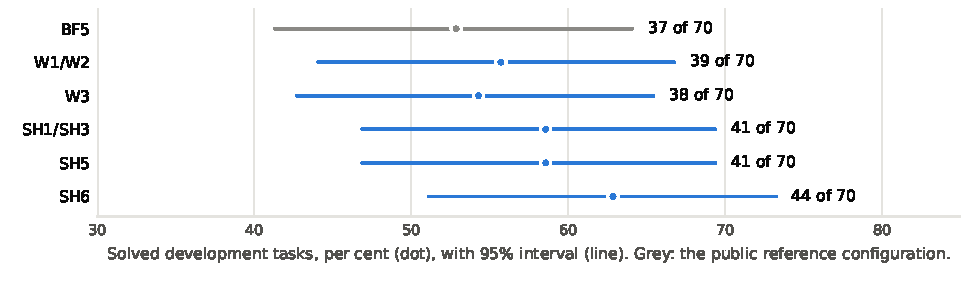
\includegraphics[width=\linewidth]{fig/pub_configs.pdf}
\caption{Six configurations of the 31B agent on the same 70 development tasks, one run per task.}
\label{fig:pub-configs}
\end{figure}

\begin{figure}[t]
\centering
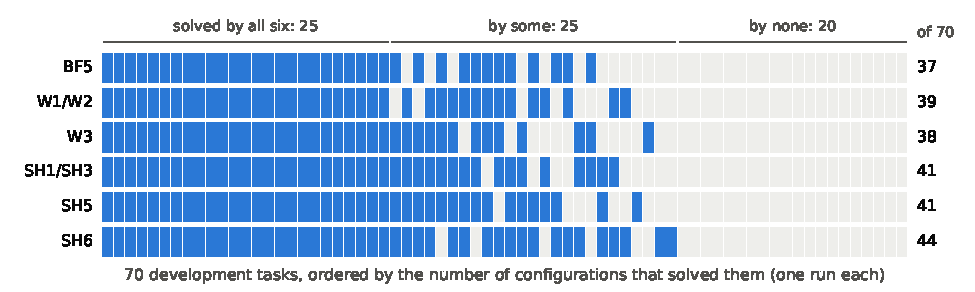
\includegraphics[width=\linewidth]{fig/pub_matrix.pdf}
\caption{Which configuration solved which task. One column per development task, one row per configuration; a filled
cell is a solved run. \PubAlwaysSix{} tasks were solved by all six configurations and \PubNeverSix{} by none.}
\label{fig:pub-matrix}
\end{figure}

\Cref{tab:pubseventy} joins the blocks into six configurations that each ran once on all 70 tasks. Two of them join
two versions of an arm: \arm{W1} on the first 30 tasks with \arm{W2} on the next 40, and \arm{SH1} with \arm{SH3}.
The six totals lie between \PubMinSeventy{} and \PubMaxSeventy{} of 70 (\cref{fig:pub-configs}). Against \arm{BF5},
the largest difference is that of \arm{SH6}, with 10 tasks that only it solved and 3 that only \arm{BF5} solved
($p = 0.09$, not corrected for the five comparisons). No difference was detected. \arm{SH6} is also the last of a series of
versions that were developed while looking at results on these same tasks, so its count is the one most exposed to
selection.

\Cref{fig:pub-matrix} shows where the configurations differ. \PubAlwaysSix{} tasks were solved by every configuration
and \PubNeverSix{} by none; on the remaining \PubBetweenSix{} tasks the outcome depends on the configuration or on the
run. The union of the six is \PubUnionSix{} tasks, against \PubMaxSeventy{} for the best single one. This gap is an
upper bound on what a choice between configurations could gain, and it is inflated: a task that one configuration
solves in half of its runs enters the union easily when six runs try it. With one run per task and configuration
the two sources cannot be separated. The experiments with E4B below therefore use repeats.

\subsection{Masked test runners}

The harness has an option that masks the test runners inside the sandbox, so that the agent cannot run the tests of
the repository. We did not know whether the hosted scorer sets it, so two arms were run on the first 30 tasks with the
runners masked (\cref{tab:masked}). \arm{BF5} solved \MaskBfMsk{} with masked runners against \MaskBfStd{} without,
and \arm{SH5} \MaskShMsk{} against \MaskShStd. The standard and the masked runs come from different blocks. No drop
was detected, and nothing in these counts suggests that the agents depend on running the tests.

\begin{table}[t]
\centering
\small
\caption{Runs with the test runners masked inside the sandbox, on the first 30 development tasks (solved of 30).}
\label{tab:masked}
\begin{tabular}{lrrrr}
\toprule
Arm & Standard & Masked & Only masked & Only standard \\
\midrule
\texttt{BF5} & 17 & 19 & 2 & 0 \\
\texttt{SH5} & 17 & 17 & 2 & 2 \\
\bottomrule
\end{tabular}
\end{table}


\subsection{Real hardware against emulated latency}\label{sec:big-real}

Two blocks on a Kaggle notebook with four L4 GPUs repeated an arm on tasks that it had run under emulated latency
(\cref{tab:lfour}). Mean time per job agreed within \LfourWallDiffFive{} and \LfourWallDiffSix\%, with the emulated
runs the slower ones, so the emulation did not make the time limit easier than it is on real hardware.

\begin{table}[t]
\centering
\footnotesize
\caption{The same arm and tasks on real 4$\times$L4 hardware (serial jobs) and under latency emulation (eight workers). Wall: mean seconds per job.}
\label{tab:lfour}
\begin{tabular}{lrrrrrrrrr}
\toprule
Arm & Tasks & Solved, L4 & Solved, emul. & Both & Only L4 & Only emul. & Wall, L4 & Wall, emul. & Diff. \\
\midrule
\texttt{SH5} & 10 & 6 & 3 & 3 & 3 & 0 & 280 & 292 & \ensuremath{-}4\% \\
\texttt{SH6} & 24 & 14 & 17 & 14 & 0 & 3 & 289 & 314 & \ensuremath{-}8\% \\
\bottomrule
\end{tabular}
\end{table}


The solved counts moved in both directions. \arm{SH5} solved \LfourRealFive{} of \LfourNFive{} tasks on real hardware
and \LfourEmuFive{} under emulation. These ten tasks had been picked as a hard mix, and three of them changed outcome
with identical agent files. \arm{SH6} solved \LfourRealSix{} of \LfourNSix{} on real hardware and \LfourEmuSix{}
under emulation. The \LfourNSix{} tasks of this second block were chosen with the earlier results of the arms in view,
which favours the emulated count; a fall on repetition is what such a choice predicts, and it is no evidence of a
difference between the machines. Neither block can support a claim about the solve rate. Together they show that a
single run per task moves by several tasks in ten to twenty-four when nothing changes.

\subsection{Berth tasks on real hardware}

Two later blocks ran 31B arms on Berth tasks on four L4 GPUs with the software stack of the scorer. The first is a
timing block with one job at a time (\cref{tab:timing}): the two public bundles and one variant of each on ten tasks.
Every arm solved 4 of 10. The agent phase took \TimingAgentMin{} to \TimingAgentMax{} seconds on average, and grading
about ten seconds.

\begin{table}[t]
\centering
\small
\caption{Timing block: four 31B arms on ten Berth tasks, jobs run one after another on 4$\times$L4 with the software stack of the scorer. Times are mean seconds per job.}
\label{tab:timing}
\begin{tabular}{lrrrrrr}
\toprule
Arm & Solved & Agent & Setup & Verify & Tokens out & Tool calls \\
\midrule
\texttt{BF5} & 4/10 & 191 & 2.9 & 10.5 & 6{,}454 & 18.5 \\
\texttt{BF5-s} & 4/10 & 233 & 4.8 & 10.1 & 7{,}710 & 19.8 \\
\texttt{ID24} & 4/10 & 193 & 3.8 & 10.7 & 6{,}551 & 16.7 \\
\texttt{ID24-r} & 4/10 & 179 & 4.0 & 7.8 & 5{,}792 & 17.1 \\
\bottomrule
\end{tabular}
\end{table}


The second block compared \arm{BF5} with \arm{BF5-c}, which adds a checking step before the patch is submitted, on 16
tasks with two repeats. \arm{BF5-c} solved \CheckCand{} of \CheckRuns{} runs and \arm{BF5} \CheckBase; \CheckUp{}
tasks gained a solved run and \CheckDown{} lost one, and the agent phase was \CheckTime\% longer. No difference was
detected.

\subsection{Hosted submissions}\label{sec:hosted}

\begin{table}[t]
\centering
\small
\caption{Our five hosted submissions (one per day) and the local result of the same configuration. The public score is the solved share on the public part of the hidden test set, as displayed.}
\label{tab:hosted}
\begin{tabular}{llllp{0.42\linewidth}}
\toprule
Date (UTC) & Arm & Model & Public score & Local result of the same arm \\
\midrule
2026-11-05 & \texttt{W3} & 31B & 0.12 & 38 of 70 development tasks (emulated latency) \\
2026-11-08 & \texttt{ID24} & 31B & 0.17 & 4 of 10 Berth tasks (4$\times$L4) \\
2026-11-09 & \texttt{base} & E4B & 0.06 & 20.2\% of 1{,}616 Berth runs (workstation) \\
2026-11-10 & \texttt{BF5} & 31B & 0.18 & 37 of 70 development tasks (emulated latency) \\
2026-11-11 & \texttt{v-a3} & E4B & 0.05 & 118 of 512 Berth runs (panel H) \\
\bottomrule
\end{tabular}
\end{table}


\begin{figure}[t]
\centering
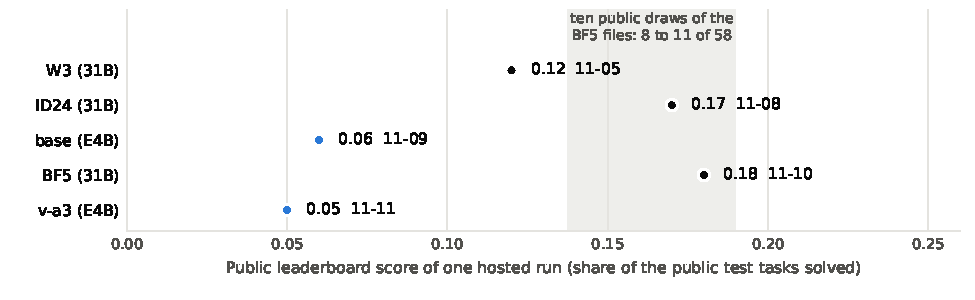
\includegraphics[width=0.9\linewidth]{fig/hosted.pdf}
\caption{Our hosted scores, one run each, against the range of ten public draws of the unchanged \arm{BF5} files
\citep{afshar2026census}.}
\label{fig:hosted}
\end{figure}

\Cref{tab:hosted} lists our five hosted submissions with the local result of the same arm. The scores are given as the
leaderboard displays them. Two of them, 0.06 and 0.18, are not a count of 58 tasks rounded to two digits, so we do
not convert scores into task counts.

Each score is one draw. The unchanged \arm{BF5} files scored between 8 and 11 of 58 in ten public draws
\citep{afshar2026census}, and our draw of these files, 0.18, lies in that range (\cref{fig:hosted}). \arm{W3} scored
0.12 and \arm{BF5} 0.18, while locally they solved 38 and 37 of the same 70 tasks. With a standard deviation near 1.5
tasks for one draw, the difference of two draws of the same files has a standard deviation near 0.04. The hosted
difference of 0.06 is about one and a half times that: it does not contradict the local tie, and it does not confirm
it. This is the situation that the
introduction describes: a difference of the size that development produces is not visible in a hosted score.

The two E4B files scored 0.06 (\arm{base}) and 0.05 (\arm{v-a3}, the third candidate of \cref{sec:programmes}). No
repeated draws of an E4B file exist, so the noise of an E4B score has not been measured. We read no direction from a
difference of 0.01 between two single draws. The local confirmation run of the same candidate (\cref{sec:confirm}) is
the evidence that we have, and its verdict is ``not confirmed''.

The local solve rates are far above the hosted scores for both models, on the development tasks and on Berth. Local
counts compare arms on the same tasks. They do not predict a hosted score.
